\section{\textbf{Additional Information}}
\vspace{-0.4mm}

\small{
\textbf{Languages:}  
\vspace{2mm}

\renewcommand{\arraystretch}{1.3} % Adjust row spacing for better readability
\begin{tabularx}{\textwidth}{>{\raggedright\arraybackslash}X c}
    % \textbf{Language} & \textbf{Proficiency} \\ \hline
    {Bangla (Native)} &  
    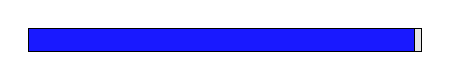
\begin{tikzpicture}
        \draw[fill=blue!90] (0,0) rectangle (4.9,0.3);
        \draw[fill=gray!20] (4.9,0) rectangle (5,0.3);
    \end{tikzpicture} \\
    
    {English (Intermediate)} &  
    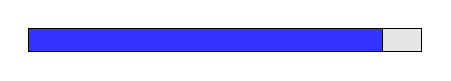
\begin{tikzpicture}
        \draw[fill=blue!80] (0,0) rectangle (4.5,0.3);
        \draw[fill=gray!20] (4.5,0) rectangle (5,0.3);
    \end{tikzpicture} \\

    {Hindi/Urdu (Basic)} &  
    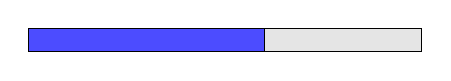
\begin{tikzpicture}
        \draw[fill=blue!70] (0,0) rectangle (3,0.3);
        \draw[fill=gray!20] (3,0) rectangle (5,0.3);
    \end{tikzpicture} \\

    % \textbf{Tripura (Native)} &  
    % \begin{tikzpicture}
    %     \draw[fill=blue!90] (0,0) rectangle (4.9,0.3);
    %     \draw[fill=gray!20] (4.9,0) rectangle (5,0.3);
    % \end{tikzpicture} \\

    % \textbf{Chakma (Native)} &  
    % \begin{tikzpicture}
    %     \draw[fill=blue!90] (0,0) rectangle (4.9,0.3);
    %     \draw[fill=gray!20] (4.9,0) rectangle (5,0.3);
    % \end{tikzpicture} \\

\end{tabularx}

\vspace{2mm}

\textbf{Interests:}  
\begin{itemize}
    \item Competitive Programming
    \item Software Development
    \item Artificial Intelligence \& Machine Learning
    % \item Open-Source Contributions
    \item Image Processing \& Computer Vision
    \item Computer Graphics
    % \item Robotics \& Embedded Systems
\end{itemize}
}
\vspace{-4mm}
